% Gemini theme
% https://github.com/anishathalye/gemini

\documentclass[final]{beamer}

% ====================
% Packages
% ====================

\usepackage[T1]{fontenc}
\usepackage{lmodern}
\usepackage[scale=1.05,size=a1]{beamerposter}
\setlength{\paperwidth}{33.1in}
\setlength{\paperheight}{23.4in}
\usetheme{gemini}
\usecolortheme{mit}
\usepackage[style=numeric,date=year]{biblatex}
\usepackage{graphicx}
\usepackage{booktabs}
\usepackage{amsmath}
\usepackage{tikz}
\usepackage{pgfplots}

\newcommand{\norm}[1]{\left\lVert#1\right\rVert}
\renewcommand*{\bibfont}{\footnotesize}
\addbibresource{poster.bib}

% ====================
% Lengths
% ====================

% If you have N columns, choose \sepwidth and \colwidth such that
% (N+1)*\sepwidth + N*\colwidth = \paperwidth
\newlength{\sepwidth}
\newlength{\colwidth}
\setlength{\sepwidth}{0.025\paperwidth}
\setlength{\colwidth}{0.3\paperwidth}

\newcommand{\separatorcolumn}{\begin{column}{\sepwidth}\end{column}}

% ====================
% Title
% ====================

\title{DeepSphere: a graph-based spherical CNN}

\author{Jules Bourcier \and Gioele Cerri \and Tony Gosse-Dumesnil}
\institute[shortinst]{Sorbonne Université -- Paris }

% ====================
% Footer (optional)
% ====================

% \footercontent{
%   \href{https://www.example.com}{https://www.example.com} \hfill
%   ABC Conference 2025, New York --- XYZ-1234 \hfill
%   \href{mailto:alyssa.p.hacker@example.com}{alyssa.p.hacker@example.com}}
% (can be left out to remove footer)

% ====================
% Logo (optional)
% ====================

% use this to include logos on the left and/or right side of the header:
\logoright{
\includegraphics[height=4cm]{su-sciences-white.png}}
% \logoleft{\includegraphics[height=7cm]{logo2.pdf}}

% ====================
% Body
% ====================

\begin{document}
\begin{frame}[t]
\begin{columns}[t]
\separatorcolumn

\begin{column}{\colwidth}
  \begin{block}{Introduction}
    The problem of treating spherical data in the context of deep learning arises in a number of different situations, such as cosmological and metereological studies.
    
    \begin{figure}[h]
      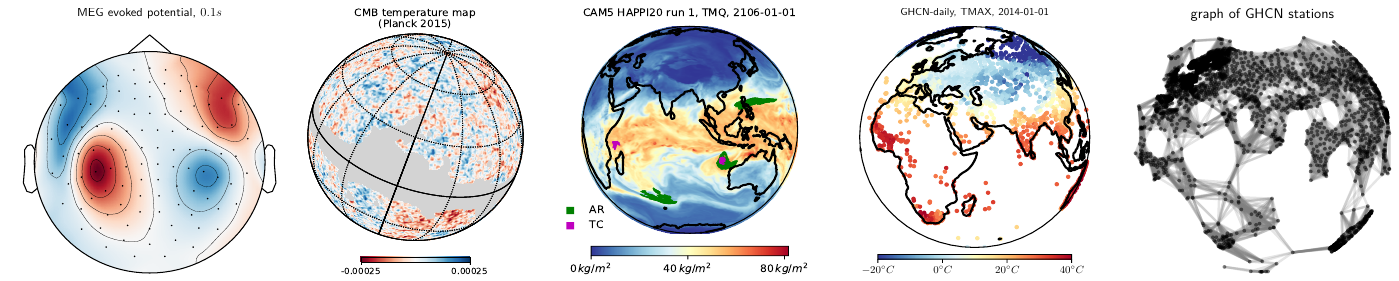
\includegraphics[width=\colwidth]{maps.png}
      \caption{Some examples of spherical data (from \cite{deepsphere_iclr:2019})}
    \end{figure}

    How can such data be modelled in order to better exploit their peculiar properties, like \emph{rotation invariance} (same output) or \emph{equivariance} (output rotated accordingly)? What strategies can be applied in order to keep the model flexible, \emph{i.e.} to control computational cost?

    The goal of this project was to implement a simple graph-based CNN as proposed by Defferrard et al. \cite{deepsphere_iclr:2019} and apply it to the problem of 3D object recognition, using the \texttt{ModelNet40} dataset \cite{modelnet}.
    The main building blocks of this network will be the operations of \emph{convolution} over a graph and \emph{pooling}.

    \begin{figure}[h]
      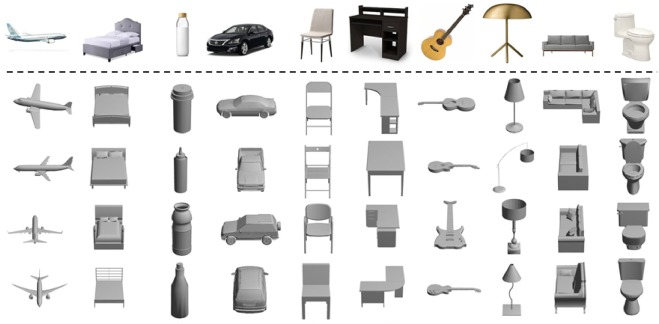
\includegraphics[width=0.7\colwidth]{modelnet40-crop.png}
      \caption{Some examples from the \texttt{ModelNet40} dataset}
    \end{figure}
  \end{block}

  \begin{block}{From the sphere to the graph}
    There are many possible \emph{projections} through which a sphere can be sampled. A natural choice for this problem is the \texttt{HEALPIX} projection, which has many interesting mathematical properties. In particular, the grid generated by the sampling is hierarchical, and the pooling operation becomes trivial.

    \begin{figure}[h]
      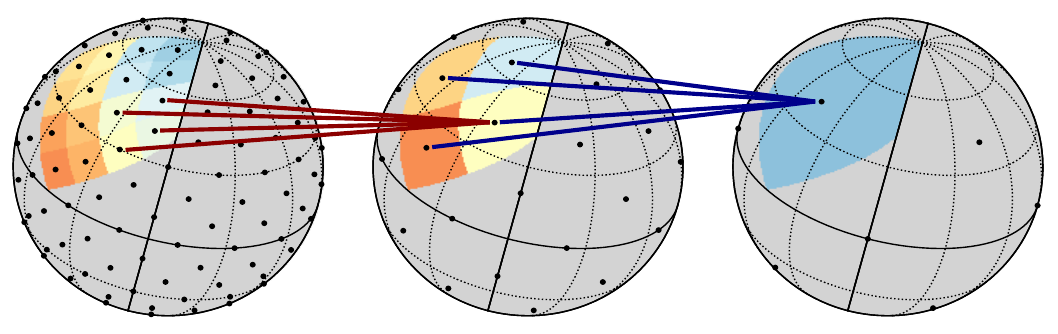
\includegraphics[width=0.7\colwidth]{healpix-pooling.png}
      \caption{The \texttt{HEALPIX} projection and pooling operation (from \cite{deepshpere_cosmo})}
    \end{figure}

    Now, a graph can be built from the spherical data: each node represents a sampling point, and it's linked with an edge to its $k$ closest points. A natural choice would be $k = 8$, but it is possible to increase the precision of the graph and reduce the equivariance error.
    
    A weight is associated to each edge, computed with the following formula:
    $$w_{ij} = \exp \left( - \frac{\norm{x_i - x_j}^2}{\rho^2} \right)$$
    $\norm{\cdot}$ is the Euclidean norm and $\rho$ is the average distance between two neighbours.
  \end{block}

\end{column}

\separatorcolumn

\begin{column}{\colwidth}

  \begin{block}{The convolution operation}
    The convolution is introduced in the Fourier space generated by the graph laplacian, which is here pictured:
    \begin{figure}[h]
      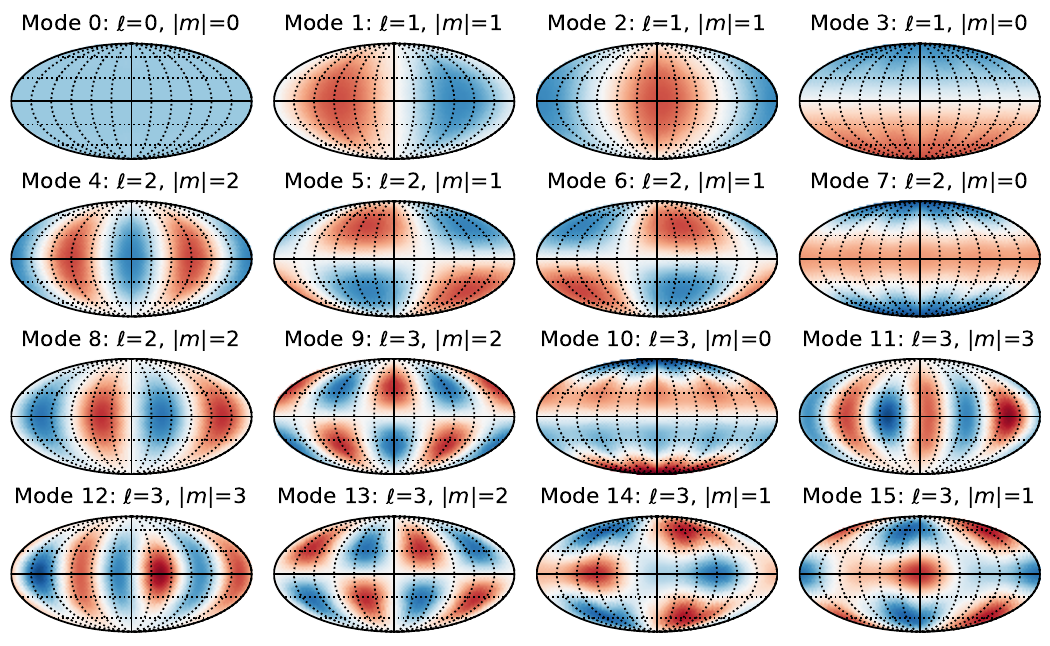
\includegraphics[width=0.7\colwidth]{healpix-fourier.png}
      \caption{Representation of eigenvectors of the \texttt{HEALPIX} graph laplacian (from \cite{deepshpere_cosmo})}
    \end{figure}
    
    To improve speed, instead of doing an exact projection on the Fourier space, the convolution will be approximated with a truncated Chebyshev expansion, whose coefficients are going to be learned as part of the network. The tradeoff between precision and speed can be controlled varying the number of coefficients $P$.
  \end{block}

  \begin{block}{CNN architecture}
    The output of the model will be the probability that a given 3D object belongs to each of the 40 classes present in the \texttt{ModelNet40} dataset.

    The dataset contains six input spherical maps for each object. A sphere which has the same center as the 3D model is constructed, and for each one of its points a radius is drawn. The distance between sphere and object forms the \emph{depth map}. Then, the two angles between the radius and the object surface are considered. Finally, the same three maps are considered with respect to the \emph{convex hull} of the object.
    \begin{figure}[h]
      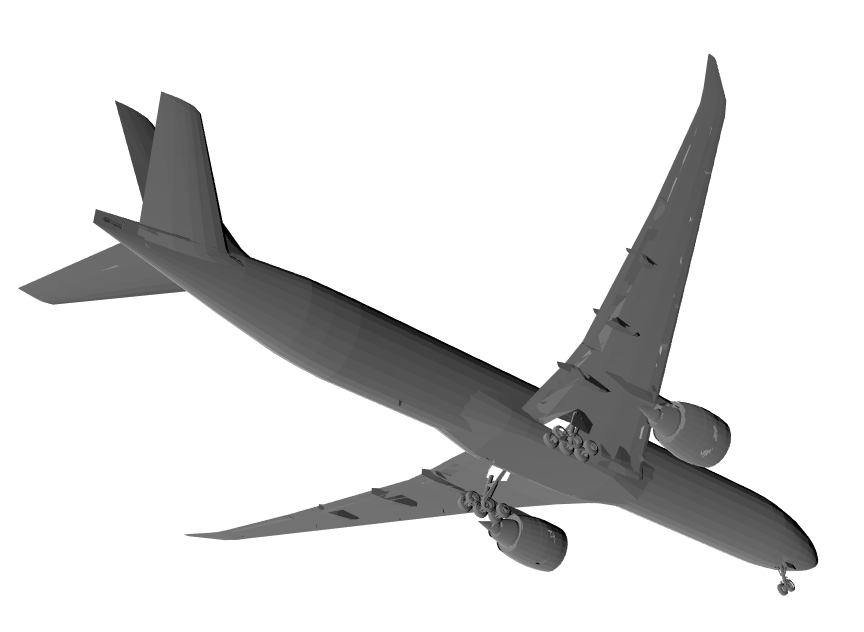
\includegraphics[height=6cm]{airplane.png}
      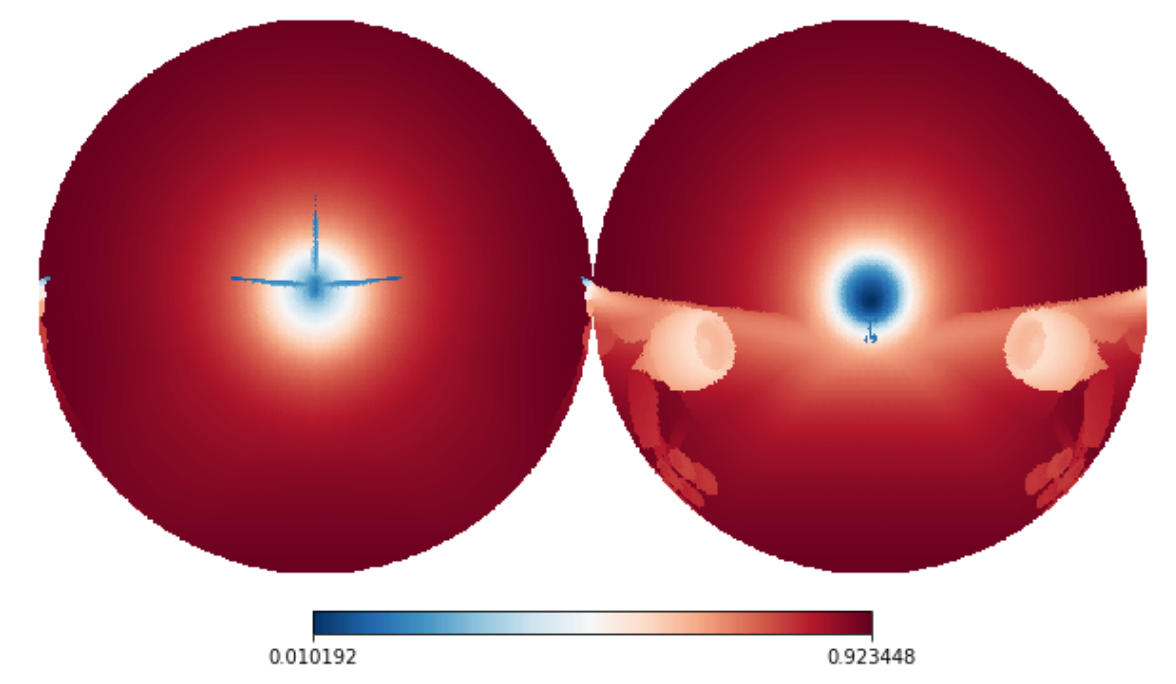
\includegraphics[height=6cm]{airplane-map.png}
      \caption{A 3D object (plane) and its depth map}
    \end{figure}

    The network consists of five convolutional layers, and a final fully-connected linear + log-softmax layer.
    % The convolutional layers are approximated with $K$ set to 6. The first one has 6 features in input, they have respectively 16, 32, 64, 64, 64 output channels, and each one of them is followed by ReLU activation and average pooling.
    The hyperparametres corresponds to the ones used in \cite{deepsphere_iclr:2019}.

    \begin{figure}[h]
      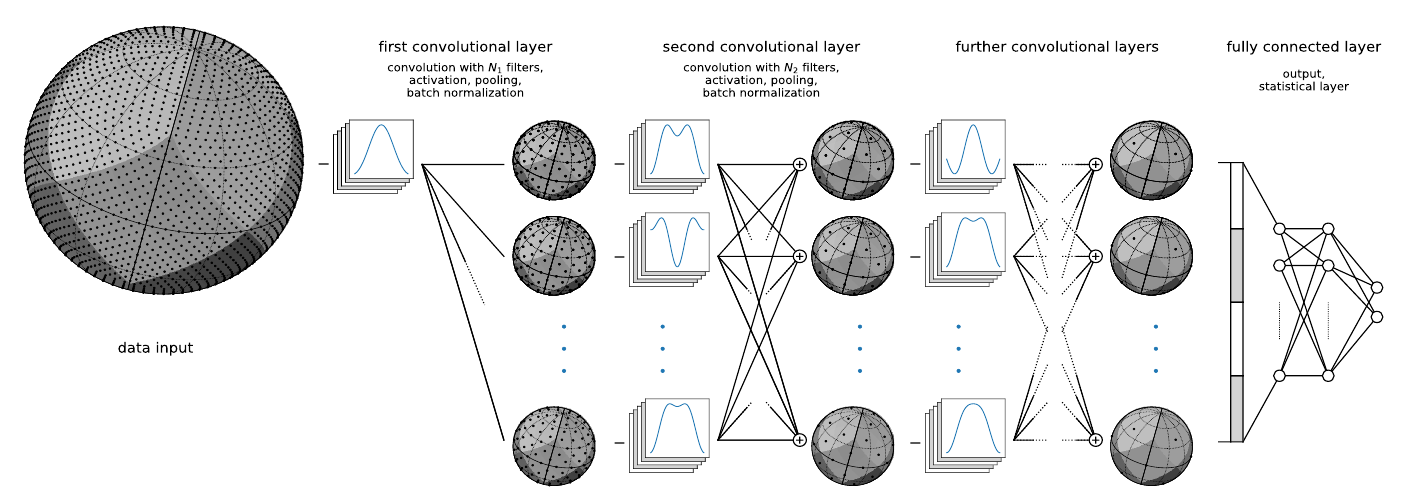
\includegraphics[width=0.9\colwidth]{scheme.png}
      \caption{Network layout (from \cite{deepshpere_cosmo})}
    \end{figure}
  \end{block}

\end{column}

\separatorcolumn

\begin{column}{\colwidth}

  \begin{block}{Results}

  \end{block}

  \begin{block}{Conclusion}

  \end{block}

  \begin{block}{References}
    \printbibliography
  \end{block}


\end{column}

\separatorcolumn
\end{columns}
\end{frame}

\end{document}
